\documentclass{article}

\usepackage[utf8]{inputenc}
\usepackage{amsmath}
\usepackage{graphicx}
\usepackage{float}
\usepackage{amsthm}

\newtheorem{theorem}{Theorem}[section]

\title{Hello YouTube!}
\author{Istvan Hegyes}
\date{2025-02-01}

\begin{document}

\maketitle

\tableofcontents
\listoffigures

\begin{abstract}
    Summmary of the document goes here.
\end{abstract}

\section{Introduction}
Let's begin with a formula $e^{i\pi}+1=0$. But we can also do

\begin{itemize}
    \item
          We can do as a \textbf{limit}:
          \begin{equation}
              \begin{aligned}
                  e & = \lim_{n \to \infty} \left(1+\frac{1}{n}\right)^n \\
                    & = \lim_{n \to \infty} \frac{n}{\sqrt[n]{n!}}       \\
                    & = \lim{t \to 0} \left(1 + t\right)^{\frac{1}{t}}
              \end{aligned}
              \label{eq:limit}
          \end{equation}
    \item
          We can write it as a \textit{sum}:
          \[
              e=\sum_{n=0}^{\infty} \frac{1}{n!} = 1 + \frac{1}{1!} + \frac{1}{2!} + \frac{1}{3!} + \frac{1}{4!} + \cdots
          \]

          We can express it as a \textit{Taylor series}:
          \begin{equation}
              e^x = \sum_{n=0}^{13} \frac{x^n}{n!} = 1 + x + \frac{x^2}{2!} + \frac{x^3}{3!} + \frac{x^4}{4!} + \cdots + \frac{x^{13}}{13!}
              \label{eq:taylor}
          \end{equation}
    \item
          We can also use \underline{continued fractions}:
          \[
              e=2+\frac{1}{1+\frac{2}{3+\frac{3}{4+\frac{4}{5+\ddots}}}}
          \]
\end{itemize}

This is equation \eqref{eq:limit}.

\section{More Formulas}

Here is an integral of a function \( f \) from \( a \) to \( b \):
\[
    \int_{a}^{b} f(x) \, dx
\]

Here is a triple integral of a function \( f \) over \( x \), \( y \), and \( z \):
\[
    \iiint_V f(x, y, z) \, dx \, dy \, dz
\]

Here is the dot product of vectors \( \vec{v} \) and \( \vec{w} \):
\[
    \vec{v} \cdot \vec{w} = \sum_{i=1}^{n} v_i w_i
\]

Here is a 3x3 matrix with the numbers from 1 to 9:
\[
    \begin{bmatrix}
        1 & 2 & 3 \\
        4 & 5 & 6 \\
        7 & 8 & 9
    \end{bmatrix}
\]

\section{Images}

Here is an example of an image:

\begin{figure}[H]
    \centering
    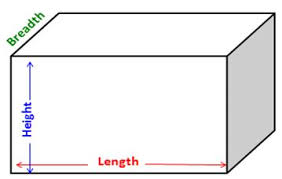
\includegraphics[width=0.5\textwidth]{images/length.jpeg}
    \caption{Definition of the length of a curve.}
    \label{fig:length}
\end{figure}
\newpage
\section{More Tricks}

\begin{table}[H]
    \centering
    \begin{tabular}{|c|c|}
        \hline
        1 & 2       \\ \hline
        3 & 4000000 \\ \hline
    \end{tabular}
    \caption{A 2x2 table with numbers 1 to 4.}
    \label{tab:numbers}
\end{table}

I like table \ref{tab:numbers}. I also like figure \ref{fig:length}.

\begin{theorem}[YouTube]
    Like and subscribe!
\end{theorem}

\end{document}